\documentclass[10pt, oneside, reqno]{amsart}
\usepackage{geometry, setspace, graphicx, enumerate}
\onehalfspacing

% AMS Theorems
\theoremstyle{plain}% default
\newtheorem{thm}{Theorem}[section]
\newtheorem{lem}[thm]{Lemma}
\newtheorem{prop}[thm]{Proposition}
\newtheorem*{cor}{Corollary}

\theoremstyle{definition}
\newtheorem{definition}[thm]{Definition}
\newtheorem{conj}[thm]{Conjecture}
\newtheorem{alg}[thm]{Algorithm}
\newtheorem{exmp}[thm]{Example}
\theoremstyle{remark}
\newtheorem*{rem}{Remark}
\newtheorem*{note}{Note}
\newtheorem{case}{Case}

\newcommand{\expc}[1]{\mathbb{E}\left[#1\right]}
\newcommand{\var}[1]{\text{Var}\left(#1\right)}
\newcommand{\cov}[1]{\text{Cov}\left(#1\right)}

\newcommand{\R}{\mathbb{R}}
\newcommand{\C}{\mathbb{C}}
\newcommand{\K}{\mathbb{K}}

\makeatletter
\renewcommand\subsection{\@startsection{subsection}{2}%
  \z@{.5\linespacing\@plus.7\linespacing}{-.5em}%
  {\normalfont\scshape}}
\makeatother

\usepackage{amsmath}	%Improves output of document containing mathematical formulas
\usepackage{amsthm}		%Enhanced version of \newtheorem command for defining theorem-like structures
\usepackage{amssymb}	%Extended symbol collection - additional binary relation symbols. Contains \amsfonts
\usepackage{amscd}
\usepackage{mathtools}	% Having piecemeal on the right hand side
\usepackage{mdframed}

\usepackage{xcolor}  % Allows the addition of colours to text
\usepackage{hyperref}
\hypersetup{
    linktoc=all,     %set to all if you want both sections and subsections linked
}
\usepackage{url}

\usepackage{graphicx}	%Allows you to insert images
\graphicspath{ {./Report/figs/} }	%Images are stored in the images folder in current directory'
\usepackage{float}
\usepackage{caption}	%Allows captions to be inserted with figures
\usepackage{listings}	%Writing code

\usepackage{algorithm} % Writing Algorithms
\usepackage[noend]{algpseudocode}

\usepackage{tcolorbox}
\tcbuselibrary{minted,breakable,xparse,skins}

\definecolor{bg}{gray}{0.95}
\DeclareTCBListing{mintedbox}{O{}m!O{}}{%
  breakable=true,
  listing engine=minted,
  listing only,
  minted language=#2,
  minted style=default,
  minted options={%
    linenos,
    gobble=0,
    breaklines=true,
    breakafter=,,
    fontsize=\small,
    numbersep=8pt,
    #1},
  boxsep=0pt,
  left skip=0pt,
  right skip=0pt,
  left=25pt,
  right=0pt,
  top=3pt,
  bottom=3pt,
  arc=5pt,
  leftrule=0pt,
  rightrule=0pt,
  bottomrule=2pt,
  toprule=2pt,
  colback=bg,
  colframe=orange!70,
  enhanced,
  overlay={%
    \begin{tcbclipinterior}
    \fill[orange!20!white] (frame.south west) rectangle ([xshift=20pt]frame.north west);
    \end{tcbclipinterior}},
  #3}
  

\title{Influentials and the Spread of Innovations}                                % Document Title
\author{Michael Lin\\470414095}

\begin{document}
\vspace*{-1.5cm}
\begin{abstract}
    This report explores the \textit{influential hypothesis} - a minority of individuals, called 
    influentials, who can spread innovations to an exceptional number of peers are important to 
    the spread of ideas/innovations. We explore this idea by performing computer simulations 
    modelling the interpersonal influence process under various conditions. It was found that 
    the importance of influentials in the spread of influence depended on the degree distribution
    of the network which suggests a reexamination of the \textit{influential hypothesis}.
\end{abstract}
\maketitle 

\section{Introduction}

The spread of influence is a well studied phenomena in social science and diffusion research 
that looks to understand how influence is spread and what factors contribute to large cascades
of influence within a population. 
This phenomena can be found in many domains such as the circulation of news by the media, the 
adoption of new technologies, and the promotion of products by social media influencers.
One hypothesis on how innovations are spread is called the \textit{influential hypothesis}\cite{Influential},
which suggests that a minority of individuals called \textit{influentials} are able to spread 
ideas/innovations to an exceptional number of peers. 
However, this model does not explain the characteristics of influentials or precisely how 
responsible they are in the cascade of influence on the (non-influential) population.

In this report, we argue that it is unclear what characteristics underpin influentials and 
whether they can be attributed to the adoption of social changes, new technologies, cultural 
fads and other diffusion processes.
By performing a series of computer simulations of various network models, it was found that 
there are instances where influentials show greater responsibility in the spread of influences.
However, under other conditions it was found that influentials are only marginally more important
than the average individual. 
Although our models are simplifications of the complexities of reality, our results highlights
the importance of population interconnectedness in dictating the responsibility of influentials
in the cascade of influence.




% In today's 

% Influentials - a minority within a population who influence an exceptional number of their peers.



\section{Interpersonal Influence Model}

For our model of the spread of influence, we assume that every individual makes a binary decision
on an innovation $X$. Moreover, we assume that the innovation exhibits \textit{positive externalities}
meaning the probability of an individual choosing $B$ over $A$ increases with the number of 
people choosing $B$. While this model is not fully generalised, as it excludes negative externality 
behaviours and innovations with multiple decisions, it is a reasonable general case to consider. 
For example, in marketing and diffusion research, positive externalities arise in many areas of 
research such as \textit{network effects}, \textit{learning from others}, and conformity 
pressures \cite{Influential}.

\subsection{Threshold Model}
A simple model to capture the aforementioned behaviour is to represent each individual $i$ by a node,
which can be in one of two discrete states $\{ 0, 1\}$, with a \textit{threshold rule} $\phi_i$. 
An individual in state $1$ is said to be influenced by an innovation while an 
individual in state $0$ is uninfluenced by an innovation.
Defining $p_i$ to be the proportion of node $i$'s neighbours who are influenced (in state $1$), then 
the probability of $i$ being influenced (in state $1$) is given by
\[ P[\text{Node } i \text{ in state } 1] = 
\begin{cases}
    1 & p_i \geq \phi_i \\
    0 & p_i < \phi_i
\end{cases} \]
where $\phi_i \in [0,1]$ refers to the minimum proportion of $i$'s neighbours that need to be 
influenced for $i$ to be influenced. Intuitively, $\phi_i$ refers to $i$'s willingness to be 
influenced.
For simplicity, we assume every node can be influenced by the same threshold rule, meaning 
for every node $i$ we have $\phi_i = \phi$ for some fixed $\phi$.

\subsection{Influence Networks}
Alongside the rule describing how individuals are able to influence each other, we also need to 
describe who influences whom.
However, social networks are not yet fully understood in terms of their network properties. 
Consequently, we make the following assumptions about our influence network for computer 
simulation.
We assume that every individual $i$ in a population of size $N$ has $n_i$ neighbours, where 
$n_i$ is drawn from an \textit{influence distribution} $p(n)$ with known average $n_{avg}$ that is much less 
than the population size $n_{avg} \ll N$.
Of note is that $n_i$ refers not to the number of individuals that $i$ knows but the number of 
other individuals they can influence due to different factors such as their character, expertise, reputation and community.
Additionally, we explore the scenario where individual influence is unidirectional, meaning 
an individual $i$ can influence its neighbour $j$ but $j$ cannot influence $i$, and 
bidirectional, meaning if $i$ can influence its neighbour $j$ then $j$ can influence $i$. 
This is to represent scenarios where an individual follows other individuals, such as Instagram 
influencers, and influence is spread in one direction and when individuals influence each 
other such as within a family.

To describe the \textit{influence distribution}, we use two common random graph models 
which contain properties similar to real social networks called Scale-Free Networks and 
Poisson Random Graphs.


\subsubsection{Poisson Random Graph}
The Poisson random graph model is a simple random graph model where the influence distribution $p(n)$ is Poisson meaning $p(n) \sim Poisson(\lambda)$ with $\lambda$ representing the average number of neighbours. In a world described by a Poisson random graph, the network exhibits no structure meaning influence connections between neighbours are random. 
Additionally, the influence distribution has little variation around its average meaning individuals who are more influential generally aren't exceptionally more influential.
With this model, connections can be either undirected or have a direction.
Consequently, this influence distribution can model worlds where the spread of influences are bidirectional or unidirectional.
% Consequently, this influence distribution can model worlds where influences are bidirectional, meaning neighbours can influence each other, and worlds where influence is unidirectional, meaning an individual can influence a neighbour but they may not necessarily influence them.

\subsubsection{Scale-Free Networks}
The scale-free random graph model is a common model which is used to simulate a network that is more reminiscent of a social network. 
Specifically, the influence distribution $p(n)$ follows a power law distribution meaning $p(n) \sim n^{-\alpha}$ for some $\alpha$.
Unlike the Poisson random graph, scale-free networks contain large hubs which represent people who are connected to a a significantly larger number of people than the average person. 
Using this model, we can more closely explore how people who can influence a larger proportion of the community compare with the average person.


\subsection{Influentials}
The characteristics of influentials is not well-defined and often described as a group who can influence an exceptional number of peers.
For our analysis, we focused on seeing whether relative high number of neighbours is a characteristic of influential people by analysing the degree of influence of subsets of the simulated population based off the number of connection of each individual.
Specifically, we analysed the following groups based off the number of connections
\[ 0-5, 5-10, 10-15, 15-20, 95-100, n_{norm} \]
where $0-5$ represents the people in the simulated data who are in the top $5\%$ ranked by number of connections and $n_{norm}$ represents the subset of the population who are at most half a standard deviation away from the average degree $n_{avg}$ of the network.




\subsection{Influence Dynamics}
For our model of influence, we implemented the following algorithm below to simulate the spread of influence\cite{github}.

\begin{enumerate}
    \item Generate a graph $G$ (Poisson/Scale-Free) of $N$ nodes, where $n_{avg}$ is known.
    \item Assign nodes to the following groups $0-5,\dots,95-100,n_{norm}$.
    \item For each group, simulate the spread of influence for each node in the group according to the following algorithm. (Spread of influence from a single node).
    \begin{enumerate}
        \item Set all nodes to state $0$ except for the initial node which is set to $1$.
        \item Simulate the spread of influence for this initial state with known threshold $\phi$.
    \end{enumerate}
\end{enumerate}

\section{Results}

Our measure of interest is the cascade size (proportion of network influenced) that can be generated by an individual within each group.
This model allows for both local and global cascades. 
Local cascades only affect a small number of individuals that are typically close to the initial influencing node. 
In contrast, global cascades can affect an exceptional number of individuals and are usually limited by the size of the population.
With this measurement, a comparison between groups can be quantified the average cascade size for each group.
Additionally, it was found that the cascade size was invariant of the population size so a population of $N=100$ was chosen due to computational limitations. Our simulations was performed for $\phi= 0.05,0.10,0.15,0.18,0.20,0.25,0.50$ and for consistency each simulation was repeated $100$ times.
 
\subsection{The Cascade Window}


The first observation made from our simulations was that the ability for a node to initiate a cascade depended significantly on the average degree for all tested networks.
Specifically, each degree distribution and choice of $\phi$ had an interval for $n_{avg}$ denoted as the \textit{cascade window} where local and global cascades are possible as seen in Figure \ref{Phi10} and \ref{Phi18}.
Outside this window, $n_{avg}$ is either too small or too high.
When $n_{avg}$ is too small, even though individuals are susceptible to influence the network isn't well connected to reach these individuals so few are influenced.
When $n_{avg}$ is too high the network is highly connected and the required number of activated neighbours needed to influence an individual meaning the initial influenced individual is unable to grow.
Additionally, while the cascade window shifts with the choice of $\phi$, the relationship between population groups remain relatively similar as seen in Figure \ref{Phi10} and \ref{Phi18}.
From this, we can conclude that the ability for an individual to influence a network depends much more on the network structure rather than the individual's personal degree of influence.


% By performing our simulation across different degree distributions, threshold values $\phi$ and average degree $n_{avg}$, it was found that 


\begin{figure}[ht]
    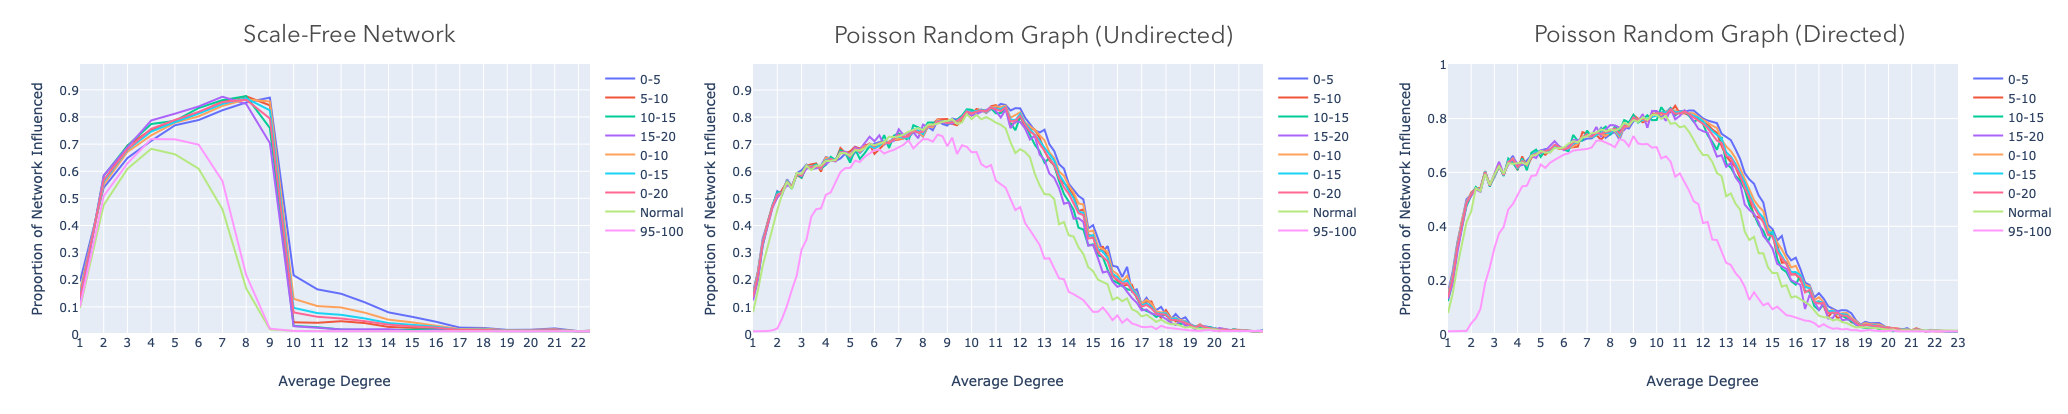
\includegraphics[scale=0.2]{Report/figs/SFRGRG10.png}
    \caption{Proportion of network influenced across different average degrees and different degree distributions with $\phi = 0.10$.}
    \label{Phi10}
\end{figure}

\subsection{Poisson and Scale-Free Influence Distributions}
The second point of interest is the comparison of cascade size between groups and between influence distributions. 
Between the directed and undirected Poisson random graph, there did not appear to be any noticeable difference in the cascade window, multiplier or cascade size across groups as seen in Figure \ref{Phi10}, \ref{Phi18}, and \ref{Mult18}.
This suggests that unidirectional and bidirectional influence relationships do not alter the spread of influence. 
Rather, it depends on the influence distribution itself which in this case is the same.



\begin{figure}[ht]
    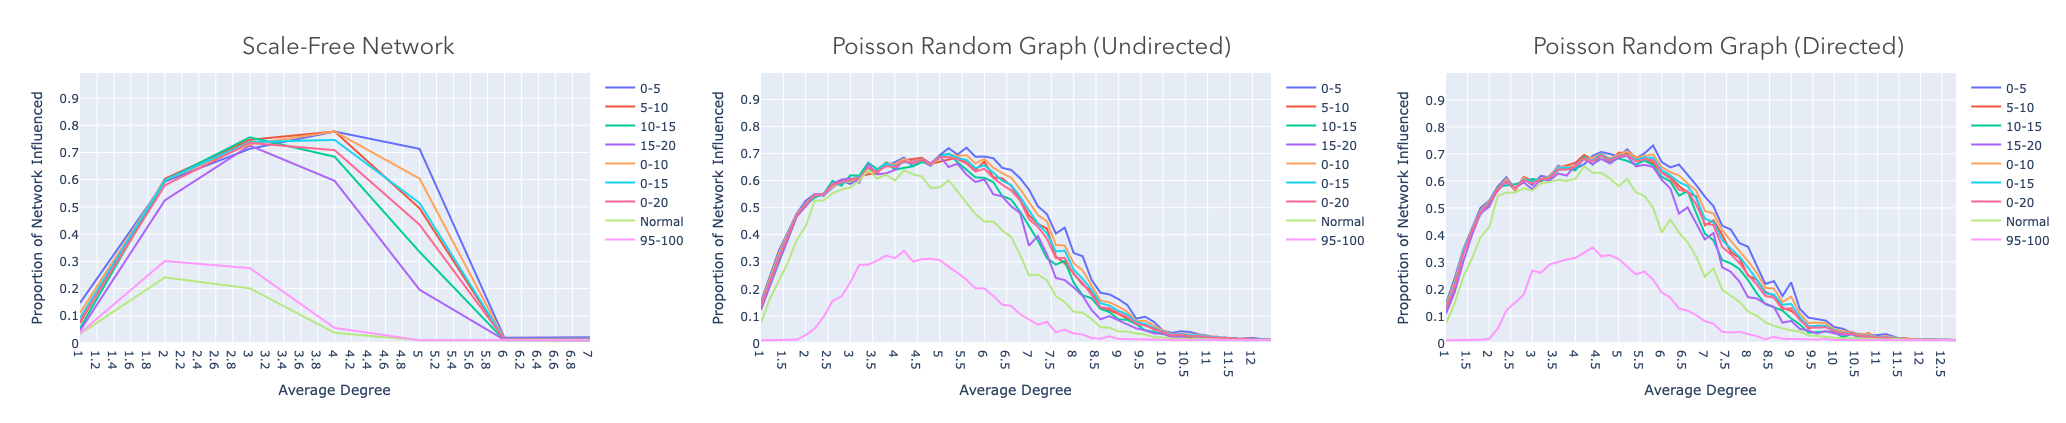
\includegraphics[scale=0.2]{Report/figs/SFRGRG18.png}
    \caption{Proportion of network influenced across different average degrees and different degree distributions with $\phi = 0.18$.}
    \label{Phi18}
\end{figure}

% Between the undirected Poisson random graph and scale-free network, 
% there are differences in the cascade window, multiplier, and cascade size across groups.

In both the Poisson random graph and scale-free network, the higher-degree groups (0-5, 5-10, 10-15, 15-20) consistently had a higher cascade size while 95-100 consistently had a noticeably smaller cascade size as illustrated in Figure \ref{Phi10} and \ref{Phi18}.
This relative comparison between groups can be associated to how being more connected (higher degree) leads to greater opportunities to influence others (higher cascade sizes) rather than the influence distribution.
Additionally, the 95-100 group can reach fewer neighbours and these neighbours are more likely to have more neighbours so they would be less susceptible to being influenced.
As the normal group generally had a cascade size lower than the higher-degree groups in both influence distributions, the relative cascade difference between higher-degree groups and the normal groups was found to quantify this difference as seen in Figure \ref{Mult18}.
In the scale-free network, the higher-degree groups compared to the normal group have a multiplier significantly greater than $1$ within the cascade window.
This suggests that higher-degree groups are much more influential than the average node and play a significant role in the spread of influence
However, the multiplier in the Poisson random graph is much more modest. In Figure \ref{Mult18}, while the multiplier peaks at around $3.8$ meaning the 0-5 cascade is typically $3.8$ times the normal group, nearing the ends of the cascade window the multiplier is much more modest suggesting that the higher-degree groups are not as significantly influential compared with the average node.
These results give mixed support for the influential hypothesis as it showcases for scale-free networks the larger role of influentials in cascades whereas in Poisson random graphs influentials have a more modest success in initiating the spread of influence.

\begin{figure}[ht]
    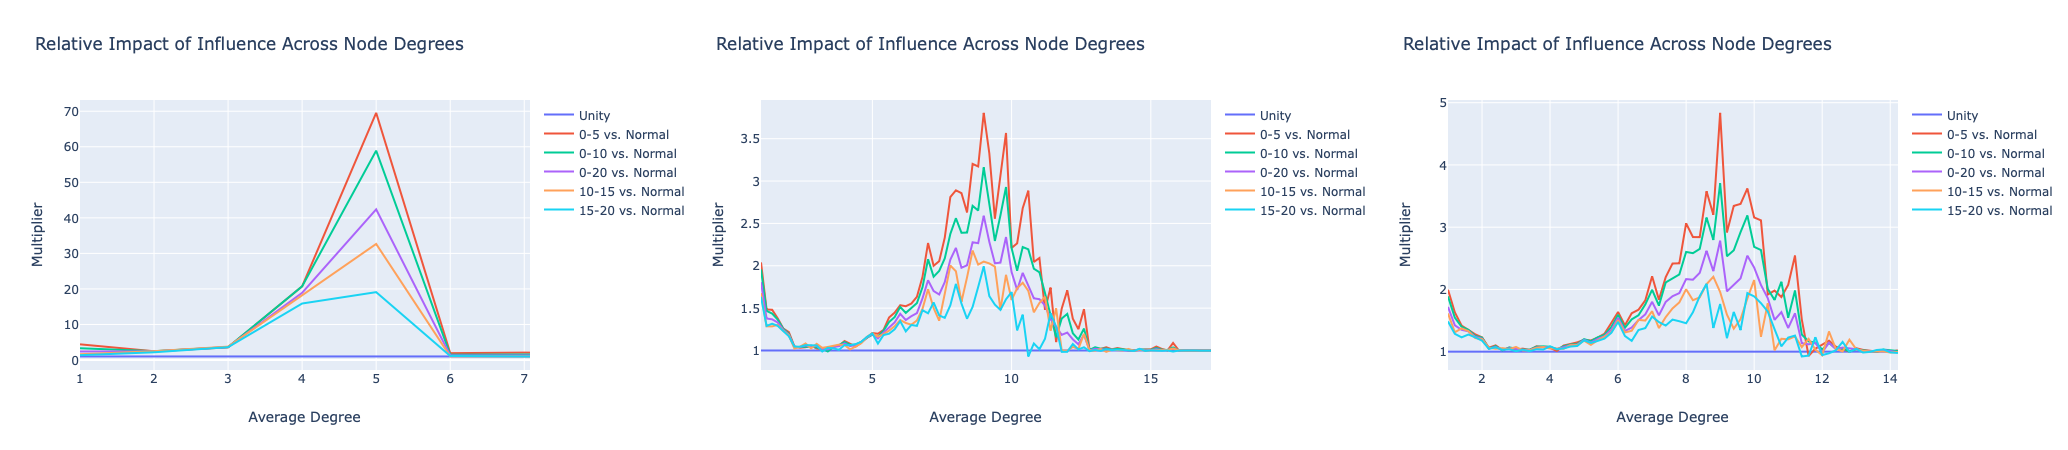
\includegraphics[scale=0.2]{Report/figs/Multiplier18.png}
    \caption{Comparison of relative cascade size between different population groups for $\phi = 0.18$. This is found by dividing cascade size between two groups. }
    \label{Mult18}
\end{figure}





% For small $\phi$ (less that $0.05$), the cascade window for scale-free networks is longer than Poisson random graphs and for large $\phi$ (greater than $0.10$), the cascade window for Poisson random graphs is longer than scale-free networks.


% \begin{itemize}
%     \item Observing the groups, consistent in both networks is the $0-5$ population having the highest cascade size across all populations within the cascade window.
%     \item The subgroups $0-5,5-10,10-15,15-20,0-10,0-15,0-20$ have similar cascade sizes between each other in both networks.
%     \item Additionally, the normal population cascade size is similar to the aforementioned subgroups for Poisson random graphs.
%     \item The normal and $95-100$ group are well separated from the other groups in scale-free networks. Unexpectedly, $95-100$ typically has larger cascade sizes than the normal group.
%     \item The $95-100$ group is well separated from the other groups in Poisson random graphs. Reason - 
%     \item By comparing the relative cascade size of the normal population and the more well-connected groups, we can compare the separation between networks. 
%     The multiplier is modest around the ends for Poisson random graphs.
%     In comparison, scale-free networks have a signifcantly larger scale which suggests that influentials play a much larger role in cascades for this kind of network.
%     This gives evidence of when influentials play an important role in the spread of influence.
%     \item The shape of the cascade size is similar across all groups in Poisson random graphs meaning each group is equally effected by changing $n_{avg}$.
%     In contrast, the normal and $95-100$ group appears to dip earlier for increasing $n_{avg}$ - associated with normal nodes having less connections and well-connected nodes being connected to less connected nodes.
% \end{itemize}

% Another point of intererest


% \begin{figure}[ht]
%     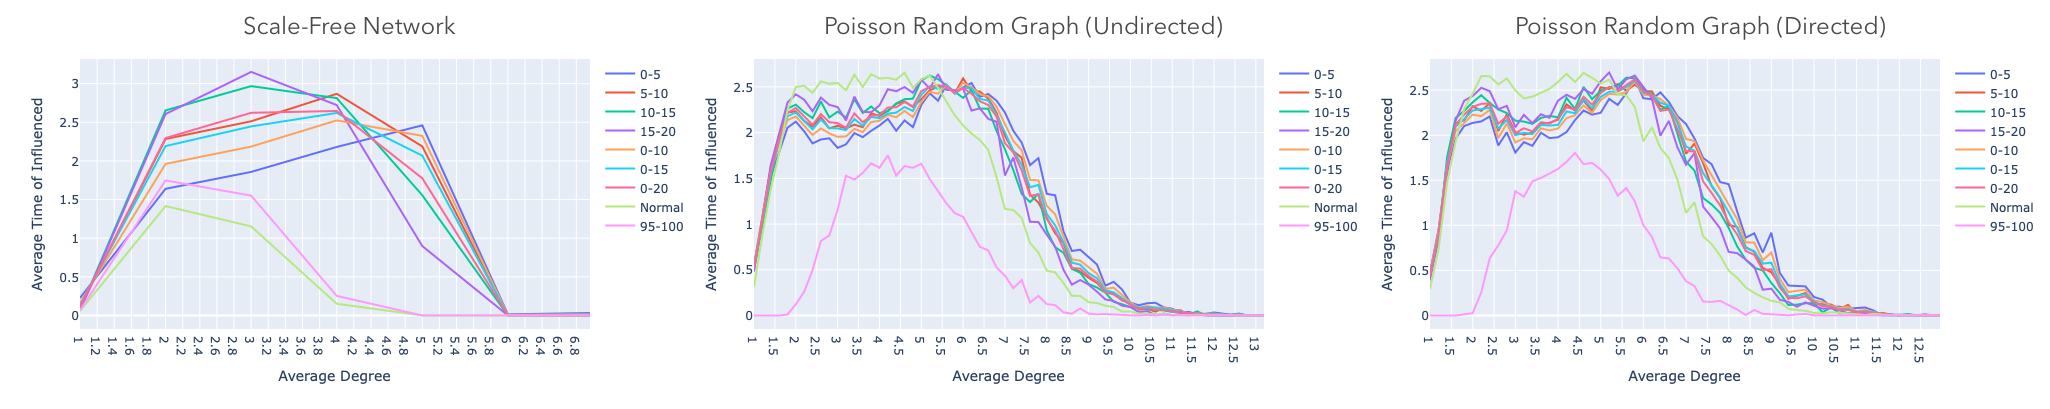
\includegraphics[scale=0.2]{Report/figs/Time18.png}
%     \caption{Comparison of average time for a node to be influenced at $\phi=0.18$.}
%     \label{Time18}
% \end{figure}

\subsection{Simulation on Real Social Networks}
Our simulation was applied on two different social networks. 
Advogato \cite{advogato} is a social community platform  where (undirected) links represent relationships between people and contained approximately $5000$ nodes. 
Facebook \cite{facebook} is a social network where (undirected) links represent friendships between people and contained approximately $4000$ nodes.
Both networks represent populations where the spread of influence can be thought of as the spread of ideas amongst friends.
Separating the nodes using the same population grouping as described above and running our simulation for the aforementioned $\phi$ values, we arrived at the results in Figure \ref{RealDat}.

% \begin{itemize}
%     \item Analysis on two datasets
%     \item Advogato\cite{advogato} is similar to Poisson random graph network
%     \item Facebook\cite{facebook} is similar to Scale-Free network
%     \item Implications on results
% \end{itemize}

\begin{figure}[ht]
    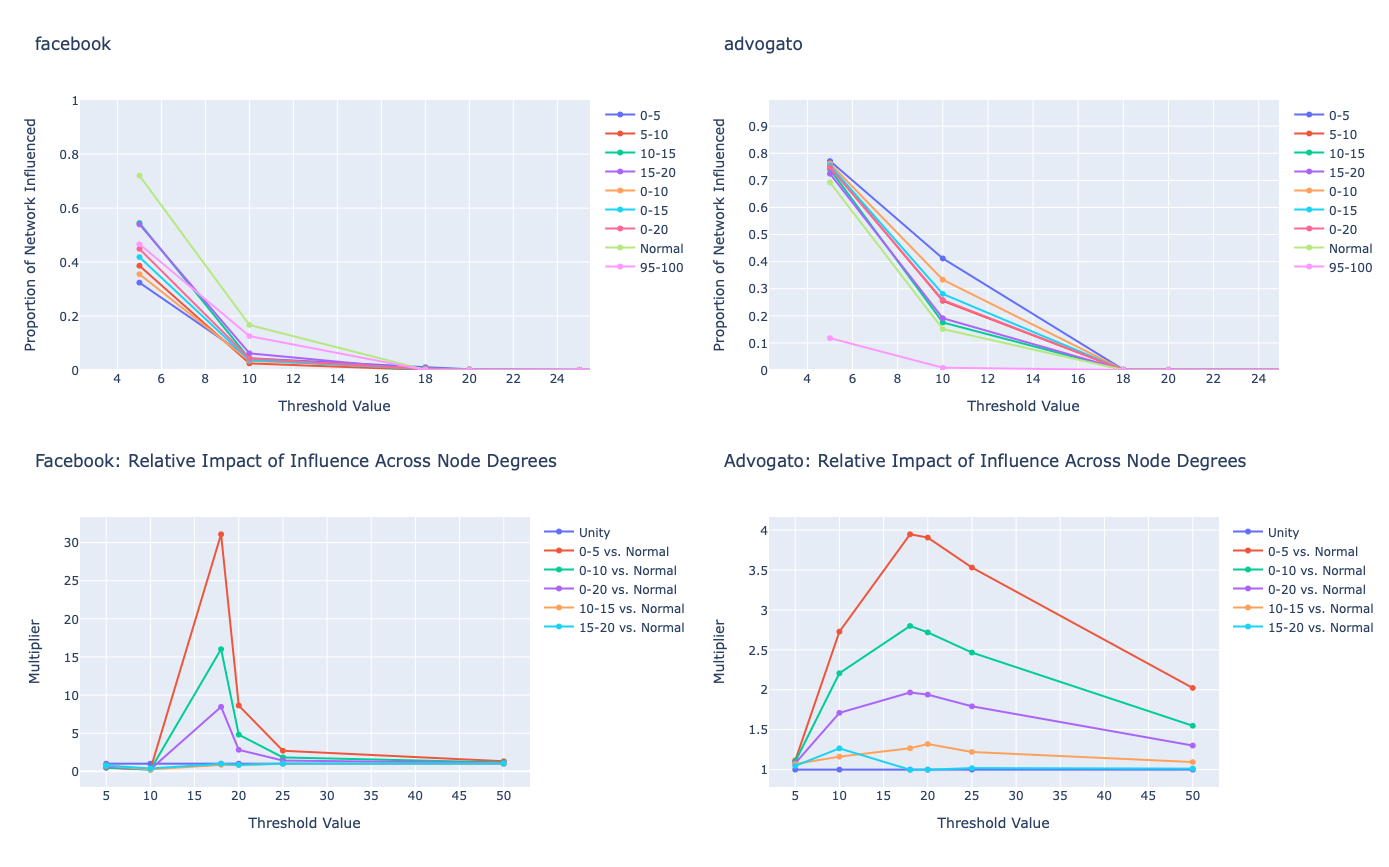
\includegraphics[scale=0.2]{Report/figs/RealDat.png}
    \caption{Application of influence simulation on two real social networks (Facebook and Advogato). The top row shows the cascade size across different $\phi$. The bottom row shows the relative cascade size between different population groups.}
    \label{RealDat}
\end{figure}

In the Facebook data, the normal group consistently outperforms all other groups in initiating cascades unlike in either of our models as seen in the Figure\ref{RealDat} (top-left).
Additionally, the 95-100 group performs similarly to the higher-degree group.
In contrast, the relative position of groups in the Advogato data is reminiscent of the Poisson (and to some extent the scale-free) as seen in Figure \ref{RealDat} (top-right).
Looking at the multiplier plots, we can see that the multiplier is generally small in both social networks (ignoring the large spike in the Facebook multiplier (bottom-left) due to a larger drop in normal cascade relative to other groups).
These results support the idea that influentials may not always play a large role in initiating cascades with the Facebook network showing the biggest cascades coming from the normal group while in the Advogato network there only appears to be a modest increase in influence for higher-degree groups.





\section{Conclusion}

In this report, it was found through simulation that an individual's role in global cascades depended more on the structure of interpersonal connections within a population rather than their degree of influence.
Specifically, there are networks (Poisson, Advogato and Facebook) where the number of neighbours that an individual can directly influence does not play a significant role in contributing to their ability to initiate or contribute to a cascade.
In other cases (such as scale-free), influential individuals play a much bigger role in initiating and spreading influence throughout the population. 
While our models are a simplification of real influence networks, the results suggest a reexamination of the influence hypothesis and motivates the exploration of other factors and attributes of influential individuals.


% \begin{itemize}
%     \item There is some truth in the impact of highly influential individuals being able to spread influence to an exceptional number of individuals.
%     \item The conditions for this depends on how well accepted the innovation is (threshold) and the interpersonal connections with the population (influence distribution). 
%     \item In some cases, relatively modest improvement in influence spread for more influential individuals but in other cases they can be an order greater as evidenced in our results and in our real social networks.
%     \item This suggests a reexamination of the notion of influence hypothesis.
%     \item Other factors and characteristics for influentials.
% \end{itemize}

\newpage
\bibliographystyle{unsrt}
\bibliography{./Report/bibliography}

\section*{Code Appendix}

The computational component of this project was done in multiple separate jupyter notebooks for the simulation component with parameter tuning and for the visualisation of the results.
This code can be found in the associated Github repository \url{https://github.com/MiLinny/Influentials}.

The code in the Github repository can be found in \texttt{/Code}.
This directory contains the code used for performing the simulations in jupyter notebooks starting with \texttt{Simulator}.
A dashboard for exploring some of the results can be found in \texttt{/Code/Dashboard.ipynb} but requires packages mentioned in the Github readme. 

Rather than overload the code appendix with all the code, this report only contains some of the helper code used for simulating the cascade of influence to give an idea. 
Note that the below implementation was adapted for cascades on a directed network. 
The whole code can be found in /Code/SimulationHelper.py of the Github repository.
The below code is split into three blocks grouped by purpose: Network Helper Functions, Simulation Helper Functions, and Simulation Functions.

\begin{itemize}
    \item Network Helper Functions: Functions used for initialising/setting influence and time attributes to the network.
    \item Simulation Helper Functions: Functions used to simulate the spread of influence such as the function simulate\_spread.
    \item Simulation Functions: Functions used for generating the graph, determining the groups of interest, running the influence cascade for each group, and summarising the results.
\end{itemize}


\newpage 
\begin{mintedbox}{python}
import networkx as nx
import numpy as np

###################################################################################
############################ Network Helper Functions  ############################
###################################################################################

def set_time(G, value, node=None, time='time'):
    '''
        Set the time of an individual node in a network G 
        to value or set the time of all nodes to value.
        G      ::  a networkx graph
        node   ::  a reference to a node in G
        value  ::  a non-negative integer
    '''
    if node:
        G.nodes[node][time] = value
    else:
        time_attrib = {i : value for i in G.nodes()}
        nx.set_node_attributes(G,time_attrib, time)
def set_influence(G, value, node=None, label='is_influenced'):
    '''
        Set the influence of an individual node in a network G 
        to value or set the influence of all nodes to value.
        G      ::  a networkx graph
        node   ::  a reference to a node in G
        value  ::  an integer 0 or 1
    '''
    if node:
        G.nodes[node][label] = value
    else:
        influence_attrib = { i : value for i in G.nodes() }
        nx.set_node_attributes(G,influence_attrib, label)
        
def get_is_influenced(G, node, label='is_influenced'):
    '''
        Returns if node in G is influenced.
    '''
    return G.nodes[node][label]
        
def get_number_influenced(G, label='is_influenced'):
    '''
        Get the number of influenced nodes.
    '''
    return sum(nx.get_node_attributes(G, label).values())

\end{mintedbox}

\begin{mintedbox}{python}
#################################################################################
########################## Simulation Helper Functions ##########################
#################################################################################

def get_uninfluenced_neighbours(G, nodes, label='is_influenced'):
    '''
        Return a set of neighbours of nodes
        that are uninfluenced.
    '''
    neighbours = set()
    for node in nodes:
        friends = list(G.neighbors(node))
        neighbours.update([friend for friend in friends if G.nodes[friend][label] == 0])
        ## implication is no node added is in nodes because nodes should all be influenced 
    
    ## In case the above implication doesn't hold...
#     tmp = set(nodes)
#     neighbours = neighbours - tmp
    return neighbours

def update_influence(G, node, phi, time, label='is_influenced'):
    '''
        Assumes the node isn't currently influenced.
        Update a node's influence status.
        Returns true or false.
    '''
    friends = list(G.neighbors(node))
    num_friends = len(friends)

    ## Node with no friends cannot be influenced
    if num_friends == 0:
        return False

    ## Calculate the number of friends who can influence 
    ## current node and compare with threshold.
    num_influenced = sum([1 for friend in friends if G.nodes[friend][label] == 1])
    if (num_influenced/num_friends) > phi:
        set_influence(G, 1, node=node)
        set_time(G, time, node=node)
        return True
    return False
    
def simulate_spread(G, initial_node, phi):
    '''
        Simulates the spread of influence from initial node under threshold phi.
        Tracks the component of influenced nodes, determines the uninfluenced 
        neighbours of this component, and determines whether the neighbours 
        can be influenced. 
        Returns the number of influenced nodes and expected time to be influenced.
    '''
    
    G_tmp = G.copy()
    set_influence(G_tmp, 1, node=initial_node)
    N = G_tmp.number_of_nodes()
    t = [0 for _ in range(N)]
    time, num_influenced = 1, 1
    t[0] = 1
    influenced_nodes = set([initial_node])
    
    ## Iteratively compute the number of nodes (update t[time]) influenced at
    ## each time step until a time step is reached where no neighbours to
    ## the influenced component can be influenced.
    while num_influenced > 0:
        num_influenced = 0
        neighbours = get_uninfluenced_neighbours(G_tmp, influenced_nodes)
        for node in neighbours:
            if update_influence(G_tmp, node, phi, time):
                num_influenced += 1
                influenced_nodes.add(node)
        t[time] = num_influenced
        time += 1
    
    ## Determine the empirical expected time to be influenced
    expected_time = sum([i * t[i] for i in range(N)])/N
    return (len(influenced_nodes), expected_time)
\end{mintedbox}

\begin{mintedbox}{python}
#################################################################################
############################# Simulation  Functions #############################
#################################################################################

def run_simulation(G, phi=0.18, q=0.1, directed=False):
    '''
        Simulation of influential cascade on network G.
        Returns the average size of influenced nodes and average expected 
        time to be influenced from 
            - influential nodes
            - normal nodes
    '''
    set_influence(G, 0)
    set_time(G, 0)
    
    degree_ordered_nodes = sorted(list(G.nodes()), key=lambda x: G.degree(x), reverse=True)
    N = G.number_of_nodes()
    degree_ordered_nodes = sorted(list(G.nodes()), key=lambda x: G.degree(x), reverse=True)
    influential_nodes_5   = degree_ordered_nodes[:int(0.05*N)]
    influential_nodes_10  = degree_ordered_nodes[int(0.05*N):int(0.1*N)]
    influential_nodes_15 = degree_ordered_nodes[int(0.1*N):int(0.15*N)]
    influential_nodes_20 = degree_ordered_nodes[int(0.15*N):int(0.2*N)]
    bottom_nodes = degree_ordered_nodes[int(0.9*N):]
    
    average = np.mean(list(dict(G.degree()).values()))
    lower, upper = int(np.floor(average)), int(np.ceil(average))
    normal_nodes = [x for x in G.nodes() if lower <= G.degree(x) <= upper ]
    
    influential_S_5, influential_S_10, influential_S_15, influential_S_20 = [], [], [], []
    influential_t_5, influential_t_10, influential_t_15, influential_t_20 = [], [], [], []
    normal_S, bottom_S = [], []
    normal_t, bottom_t = [], []
    
    ## Calculate the number of influenced nodes (S) and expected time of influenced nodes
    ## for each influential node
    for node in influential_nodes_5:
        S, t = simulate_spread(G, node, phi)
        influential_S_5.append(S)
        influential_t_5.append(t)    
    for node in influential_nodes_10:
        S, t = simulate_spread(G, node, phi)
        influential_S_10.append(S)
        influential_t_10.append(t)
    for node in influential_nodes_15:
        S, t = simulate_spread(G, node, phi)
        influential_S_15.append(S)
        influential_t_15.append(t)
    for node in influential_nodes_20:
        S, t = simulate_spread(G, node, phi)
        influential_S_20.append(S)
        influential_t_20.append(t)
    for node in bottom_nodes:
        S, t = simulate_spread(G, node, phi)
        bottom_S.append(S)
        bottom_t.append(t)
    for node in normal_nodes:
        S, t = simulate_spread(G, node, phi)
        normal_S.append(S)
        normal_t.append(t)

    return [np.mean(influential_S_5), np.mean(influential_S_10), np.mean(influential_S_15), np.mean(influential_S_20), np.mean(influential_S_5 + influential_S_10), np.mean(influential_S_5 + influential_S_10 + influential_S_15), np.mean(influential_S_5 + influential_S_10 + influential_S_15 + influential_S_20), np.mean(normal_S), np.mean(bottom_S),
            np.mean(influential_t_5), np.mean(influential_t_10), np.mean(influential_t_15), np.mean(influential_t_20), np.mean(influential_t_5 + influential_t_10), np.mean(influential_t_5 + influential_t_10 + influential_t_15), np.mean(influential_t_5 + influential_t_10 + influential_t_15 + influential_t_20), np.mean(normal_t), np.mean(bottom_t)]
\end{mintedbox}


% \section{Main Points}

% \begin{itemize}
%     \item Influentials - a minority within a population who exert influence on an exceptional number of their peers.
%     \item Motivation - We want to understand whether influentials play a significant role in the spread of influence.
%     \item How - What factors within a network contribute to the spread of innovations and does it affect the influence of influentials
%     \item 
% \end{itemize}


% Background 
% \begin{itemize}
%     \item What are influentials 
%     \item 
% \end{itemize}

% \begin{itemize}
%     \item Poisson Random Graph - If a cascade can occur, anyone can start it
% \end{itemize}

% \section{Introduction}

% \subsection{The Influentials Hypothesis}
% \texttt{Influentials} are a minority of individuals who influence an exceptional 
% number of their peers. 

% The \textbf{hypothesis} was that influentials were mediators between the source of innovation and the majority 
% of society. The model, called the \texttt{two-step flow} of communication.

% \subsection{Questions of Interest}
% \begin{itemize}
%     \item What does the two-step model say about influentials?
%     \item How do influentials exert influence over the larger population?
%     \item Are influentials responsible for the spread/diffusion of innovation?
% \end{itemize}




% \subsection{General Results}

% \begin{itemize}
%     \item Under certain (rare) conditions, influentials appear responsible for 
%     initiating cascades of influence and are important.
%     \item Under most conditions, most cascades are driven by easily influenced individuals
%     influencing other easily influenced individuals.
% \end{itemize}


% \begin{itemize}
%     \item Model: Two-way influence model with influentials acting as a middle-man.
%     \item Simulations suggest that under certain conditions, influentials promote 
%     cascading effects but these conditions are rare.
%     \item Computer simulation models 
% \end{itemize}


% Simulations 

% Threshold Model
% \begin{itemize}
%     \item Each individual $i$ in a population of $N$ influence $n_i$ random individuals.
%     \item Early adopters are individuals who adopt an innovation when a single neighbour has innovated.
% \end{itemize}




\end{document}



